%!TEX root = practicum2.tex
The performance of the perceptron trained with the Minover algorithm can be measured using the generalization error defined in \autoref{eq:method:generalization_error}. To explore the behaviour of the Minover algorithm discussed in section \ref{s:method} we have tested a perceptron trained with this algorithm on several $N$-dimensional datasets with $P = \alpha N$, for $N = 10$ and $\alpha = 0.1, 0.2, \dotsc, 5$. To ensure that the dataset was linearly separable we have determined its labels via \eqref{eq:method:teacher_label}, using the weight vector $\vec{w}^* = [1, \dotsc, 1]^T$.\\

\begin{figure}[b]
	\centering
	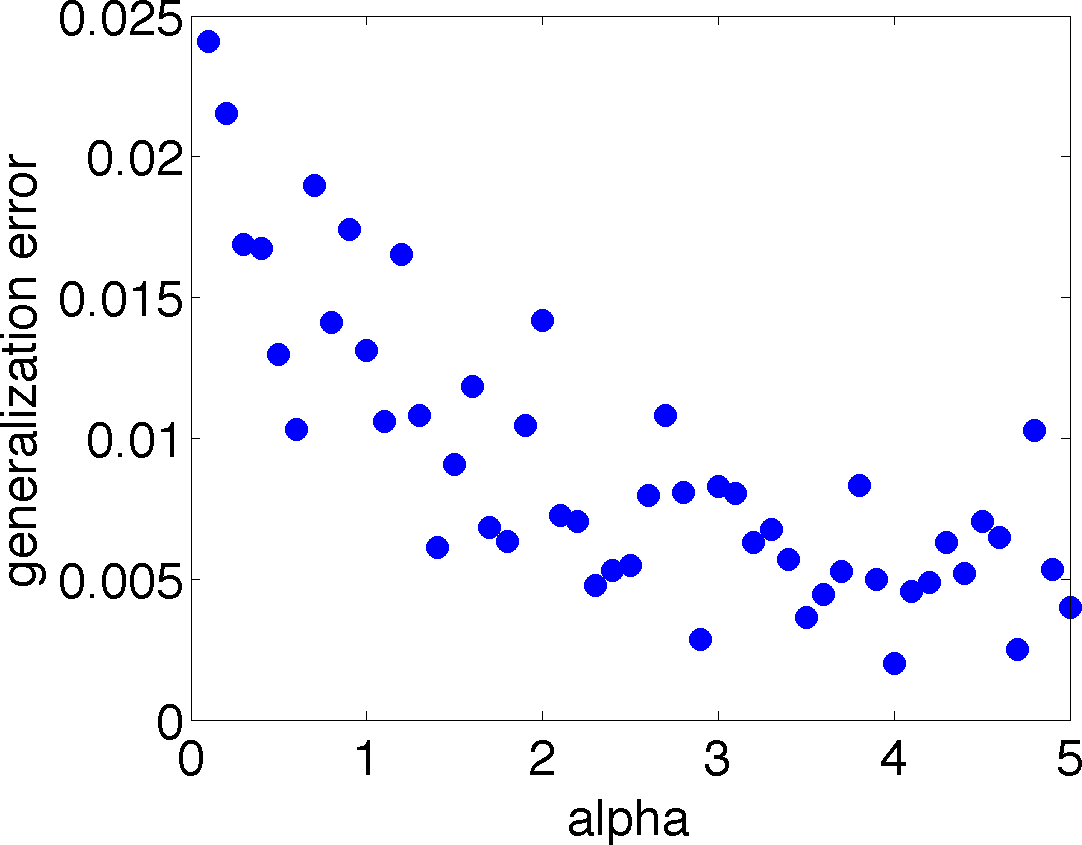
\includegraphics[width=0.9\columnwidth]{./img/finalgeneralizationerrors}
	\caption{Generalization error at the final step of training as an average of twenty iterations for $\alpha = 0.1, 0.2, \dotsc, 5$, $\varepsilon = 0.0005$, $n_{max} = 500$ and $N = 10$.}
	\label{fig:exp:finalgeneralizationError}
\end{figure}

\Cref{fig:exp:finalgeneralizationError} shows the generalization error, between the student and teacher perceptron, for different values of $\alpha$ as an average of $n_d = 20$ iterations with each $\alpha$. We consider a generalization error final when it has converged or when $t_{max}$ has been reached as explained in \cref{s:method}. 

Based on \cref{fig:exp:finalgeneralizationError} we can state that the generalization error decreases as $\alpha$ increases. A small $\alpha$ results in a smaller number of patterns, this means that it is more probable that the teacher is not the optimal solution. Because of this the generalization error is likely to be larger than with a large $\alpha$ which results in a larger number of patterns and less possible solutions, thus meaning a higher probability the teacher lies near (or is) the solution with maximum stability.

The fluctuations in the $\epsilon_g$ in \cref{fig:exp:finalgeneralizationError} may be due to the random data sets.\\
